\section{Extraction de l'information}
L'extraction se compose des phases de segmentation du texte, de la reconnaissance des entités nommées (REN), de l'analyse des relations entre entités. Toutes les étapes qui extraient, d'une manière ou d'une autre, de l'information depuis le document source ou d'un fragment de celui-ci. 
La finalité des opérations d'extraction de l'information dans le cadre de ce processus est de fournir un tableau de données, ou un système de table de données, reprenant toutes les informations semi-structurées du document source mises sous forme structurée, de sorte que ces données puissent directement servir à des études quantitatives.

\subsection{Segmentation du texte}
La segmentation du texte est l'une des premières phases du processus. Comme déjà expliqué, les rentes sont ordonnées dans le registre en fonction d'éléments topographiques (escroete, connétablie, rang de voie) et chacun de ces éléments topographiques est renseigné par un marqueur de structure. Deux précisions  importantes : premièrement, ces les éléments topographiques représenté par ces marqueurs sont hiérarchisé; secondement, chacun de ces marqueurs de structure est unique\footnote{A l'exception des marqueurs de rang de voie.}.
Cela signifie, d'une part, que les rentes sont toujours situés dans une connétablie, elle-même, au sein d'une escroete et d'autres part, qu'une rente ne peut appartenir qu'à une et une seule connétablie, au même titre qu'une connétablie ne peut appartenir qu'à une et une seule escroete.
Le cas des indications de rang de voie est plus particulier dans le sens où selon la nature de la connétablie - qui n'est pas dans tout les cas une rue disposant de deux rangées de propriétés bâties - elle peut ne pas être et que les rangs de voies ne disposent pas d'identification unique.
Les marqueurs étant chacun uniques, ils constituent des clés idéales pour identifier une rente ou un groupement de rentes en fonction d'un élément topographique. 

C'est donc sur base de la reconnaissance de ces marqueurs par des \textit{regex}\footnote{appelées aussi \og expressions régulières\fg{}.} que l'algorithme va, de manière récursive, découper le texte initial en plusieurs parties. Dans un même temps, l'algorithme va construire un tableau de données afin de  recueillir les informations. 

La figure 2.1 illustre par un organigramme les étapes effectuées par le script de segmentation du texte source.
l'algorithme va en premier lieu parcourir le fichier et indexer tout les marqueurs d'escroete. Pour chaque marqueur d'escroete indexé, la section concernant celle-ci, ainsi que la définition, vont être capturées et stockées dans un tableau de données\footnote{appelé aussi \textit{dataframe}, ou \textit{df} en abrégé}. Maintenant que le document texte est découpé au niveau des marqueurs d'escroete, pour chaque escroete répertoriée dans le tableau de données, une fonction similaire va être appelée  en prenant comme argument la section de l'escroete concernée au lieu du texte source. La fonction va donc détecter et indexer les marqueurs de connétablie. Ensuite pour chaque marqueurs de connétablie indexé, la section va capturer et stocker dans un nouveau  tableau de données et pour chacune des connétablies, à nouveau, une fonction similaire va être appelée pour effectuer les mêmes opérations : indexation des marqueurs, capture et stockage des sections, au niveau des rangs de voie, puis encore une fois au niveau des rentes.

Une fois la section de toutes les rentes d'un rang de voie stockées dans un tableau de données avec leur clé\footnote{
La clé prend la valeur du marqueur, dans le cas des rentes il s'agit du numéro de rente}, la fonction appelée renvoie ce tableau à la fonction appelante. Soit la fonction d'extraction des rang de voie, si la connétablie en possède, soit directement la fonction d'extraction des connétablies dans l'autre cas. La fonction appelante va collecter tous les tableaux - un pour chacune des sections qu'elle stocke dans son propre tableau de données - et va ensuite les fusionner en y rajoutant sa propre clé (indicateur du rang de voie ou numéro de connétablie). L'opération est répétée ensuite vers les fonctions appelantes supérieures.

De l'exécution du script résulte au final un tableau de données contenant la clé et la définition de chaque escroete, de chaque connétablie, et de chaque rente. La création d'un système de tables de données à la place d'un grand tableau de données a également été envisagé, cependant la solution du tableau de données a été retenu pour sa plus grande simplicité de mise en place et d'utilisation pour et parce qu'elle était suffisante pour les besoins du projet. L'alternative du système de table de données sera abordée avec plus de précision  dans la partie \textit{Discussion} du mémoire.

\begin{figure}[ht] % insère une figure ici (h = "here")
    \centering
    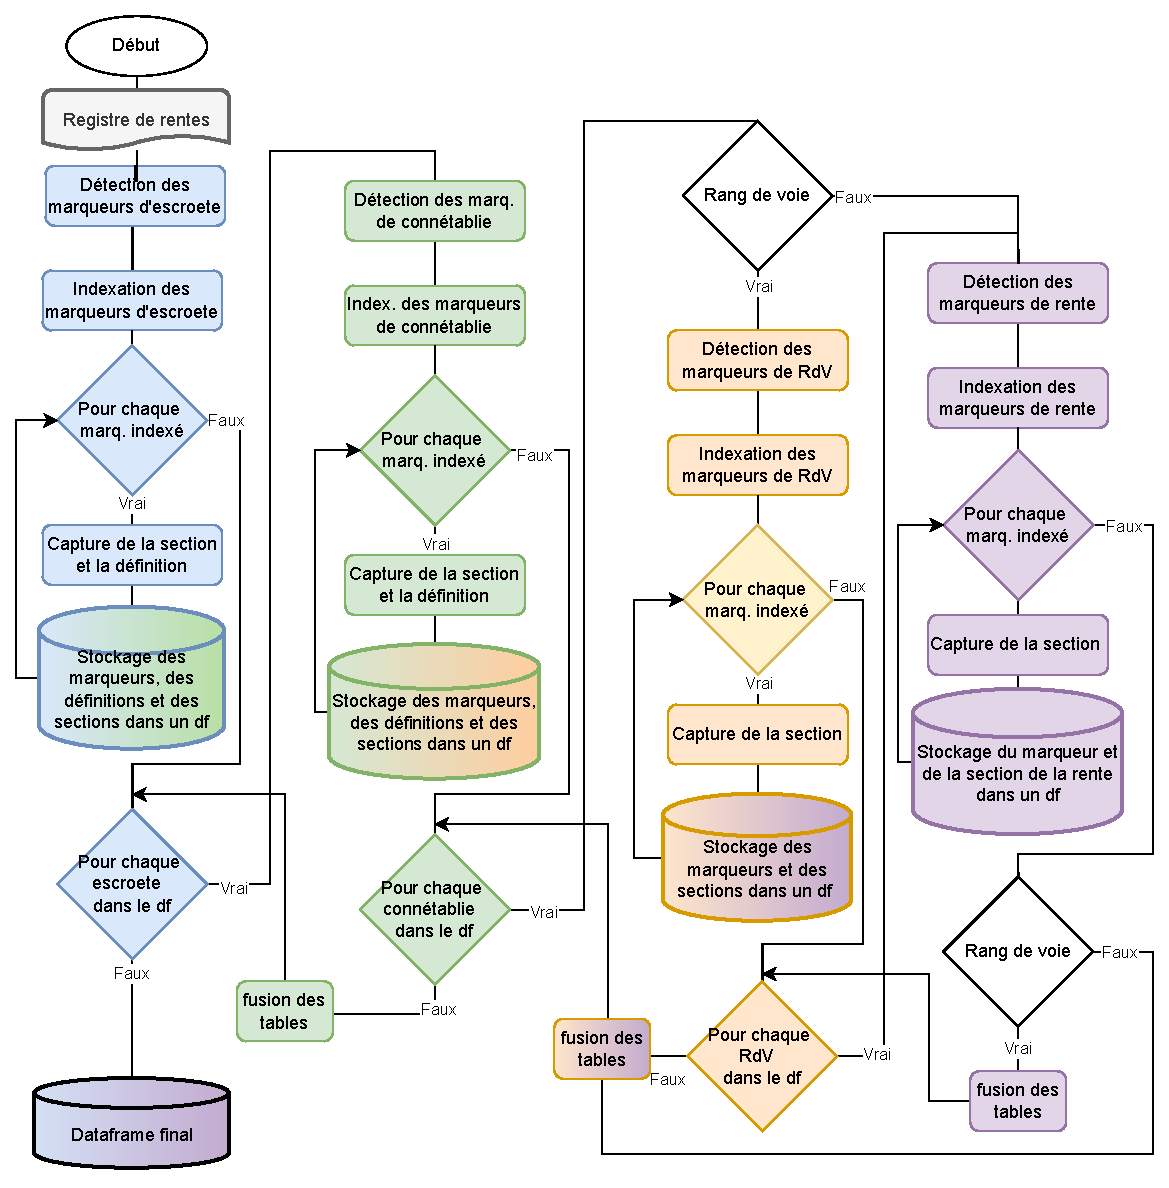
\includegraphics[scale=0.75]{2.Methods/Img/seg.drawio.pdf} 
    \caption{Organigramme de la segmentation automatisée du registre de rente.}
\end{figure}


\subsection{Reconnaissance et extraction des entités nommées}

\subsection{Analyse des relations entre entités}